%\documentclass[british, titlepage, oneside]{ntnuthesis}
\documentclass[british, oneside]{ntnuthesis}

\usepackage{import}
\usepackage{preamble/head_mk2}  % import allows for self made .sty files

% Save the document enviroment to for saving to github
% Turn on or off by setting the state of the boolean variable
% To save without the chapter content, update the .gitgnore file with filenames

\newif\ifSaveGit
\SaveGitfalse  % \SaveGittrue sets the state of the boolean variable \ifdothat` to true, o.w. it's false already (or use \dothatfalse explicitly)

% --- Import support files --- %
    
% From https://www.overleaf.com/learn/latex/Glossaries

\makeglossaries % Prepare for adding glossary entries


\newglossaryentry{latex}
{
        name=latex,
        description={Is a mark up language specially suited for
scientific documents}
}

\newglossaryentry{bibliography}
{
        name=bibliography,
        plural=bibliographies,
        description={A list of the books referred to in a scholarly work,
typically printed as an appendix}
}

\newglossaryentry{maths}
{
    name=mathematics,
    description={Mathematics is what mathematicians do}
}


% --------------------
% ----- Acronyms -----
% --------------------

\newacronym{phd}{PhD}{philosophiae doctor}
\newacronym{CoPCSE}{CoPCSE@NTNU}{Community of Practice in Computer ScienceEducation at NTNU}
\newacronym{gcd}{GCD}{Greatest Common Divisor}
  % add glossary and acronym lists before document
    
%% Commands for the document
%% ---------------------------------------------------------------------

% Defines a new command for the horizontal lines, change thickness here
\newcommand{\HRule}{\rule{\linewidth}{0.5mm}} 
%\renewcommand{\arraystretch}{1.25}



%% Mathematical symbol commands
%% ---------------------------------------------------------------------
%\newcommand{\N}{\mathbb{N}}  % Already defined
\newcommand{\Z}{\mathbb{Z}}
\newcommand{\bbP}{\mathbb{P}}
\newcommand{\PP}{\mathbb{PP}}
\newcommand{\Q}{\mathbb{Q}}
\newcommand{\R}{\mathbb{R}}
%\newcommand{\C}{\mathbb{C}}  % Already defined
\newcommand{\Fp}{\mathbb{F}_p}
\newcommand{\Fq}{\mathbb{F}_q}


\newcommand{\Tau}{\mathrm{T}}

%% Z med striketrhough
\newcommand{\Zstroke}{\text{\ooalign{\hidewidth\raisebox{0.2ex}{--}\hidewidth\cr$Z$\cr}}}
\newcommand{\zstroke}{\text{\ooalign{\hidewidth -\kern-.3em-\hidewidth\cr$z$\cr}}}



\newcommand{\degc}{$^\circ$C~}
\renewcommand{\deg}{\ensuremath{^{\circ}}}
\newcommand{\edegc}{^\circ \text{C}~}
\newcommand{\minone}{$^{-1}$}
\newcommand{\eminone}{^{-1}}



%% Other Settings
%% ---------------------------------------------------------------------
% \masl{m.a.s.l}


% --- Macros --- %
% User defined macros (functions) can go here, 
% these may be overriden for each subfile by using \renewcommand{}[][]{}
\newcommand{\set}[1]{\{#1\}} % A macro for making a set

%% normal-brackets
\newcommand{\brac}[1]{\left(#1\right)}
%% Square-brackets
\newcommand{\bras}[1]{\left[#1\right]}
%% Curly-brackets
\newcommand{\braq}[1]{\left\{#1\right\}}


\newcommand{\spn}[1]{\operatorname{span}\left( #1 \right)}
\newcommand{\spnclos}[1]{\overline{\operatorname{span}}\left( #1 \right)}
\newcommand{\mes}[1]{\operatorname{mes}\left( #1 \right)}  % same but for commands
    
    % Bibliography file
    %\addbibresource{support_files/Mastergrad.bib}

    \ifSaveGit
        \addbibresource{support_files/x_lorum_biblio.bib}
    \else
        \addbibresource{support_files/Mastergrad.bib}
    \fi % Outer \fi
% ---



% title if using "titlepage" option in documentclass
%

%\title{An NTNU Thesis \LaTeX{} Document Class}
%\shorttitle{An NTNU Thesis Document Class}
%\author{CoPCSE$@$NTNU \& Thomas Wilskow Thorbjørnsen}
%\shortauthor{CoPCSE$@$NTNU \& TWT}
%\date{\today}


\title{Plaser din fancy lange tittel her}
\shorttitle{Masteroppgave}
\author{Max Hauge}
\shortauthor{MH}
\date{\today}

\begin{document}

    % --- Preliminaries --- %
    % Title for the document
% --------------------------------------------------------------------------

\begin{titlepage}
	\makeatletter
	\let\thetitle\@title
	\let\theauthor\@author
	\let\thedate\@date
	\makeatother

	\centering
    \vspace*{0.5 cm}
    % University Logo
    
\includegraphics[width=0.7\textwidth]{ntnu.png}\\[1.0 cm]
    
	% University Name
	\textsc{\LARGE \textsf{\NTNULowerC}}\\[1.0 cm]  %* sans serif no caps
	%\textsc{\LARGE \textsf{\NTNU}}\\[1.0 cm]  %* sans serif caps
    %\textsc{\LARGE \NTNU}\\[1.0 cm]  %* RM caps
    
	% Institute
	\textsc{\Large \textsf{\NTNUinstituttLowerC}}\\[0.5 cm]  %* sans serif no caps
    %\textsc{\Large \NTNUinstitutt}\\[0.5 cm]  %* RM caps
	
	% Course Name
	\textsc{\large \textsf{\emnekode}}\\[0.5 cm]  %* sans serif no caps
	%\textsc{\large \emnekode}\\[0.5 cm]  %* RM caps
	
	%------------
	\rule{\linewidth}{0.2 mm} \\[0.4 cm]
	{ \LARGE \textbf{\textsf{\uppercase{\thetitle}}}}\\
	\rule{\linewidth}{0.2 mm} \\[1.0 cm]%[1.5 cm]
	
	

%! When the figure is used in the title, the figure environment is removed

%\begin{figure*}[h!]
%    \centering
    %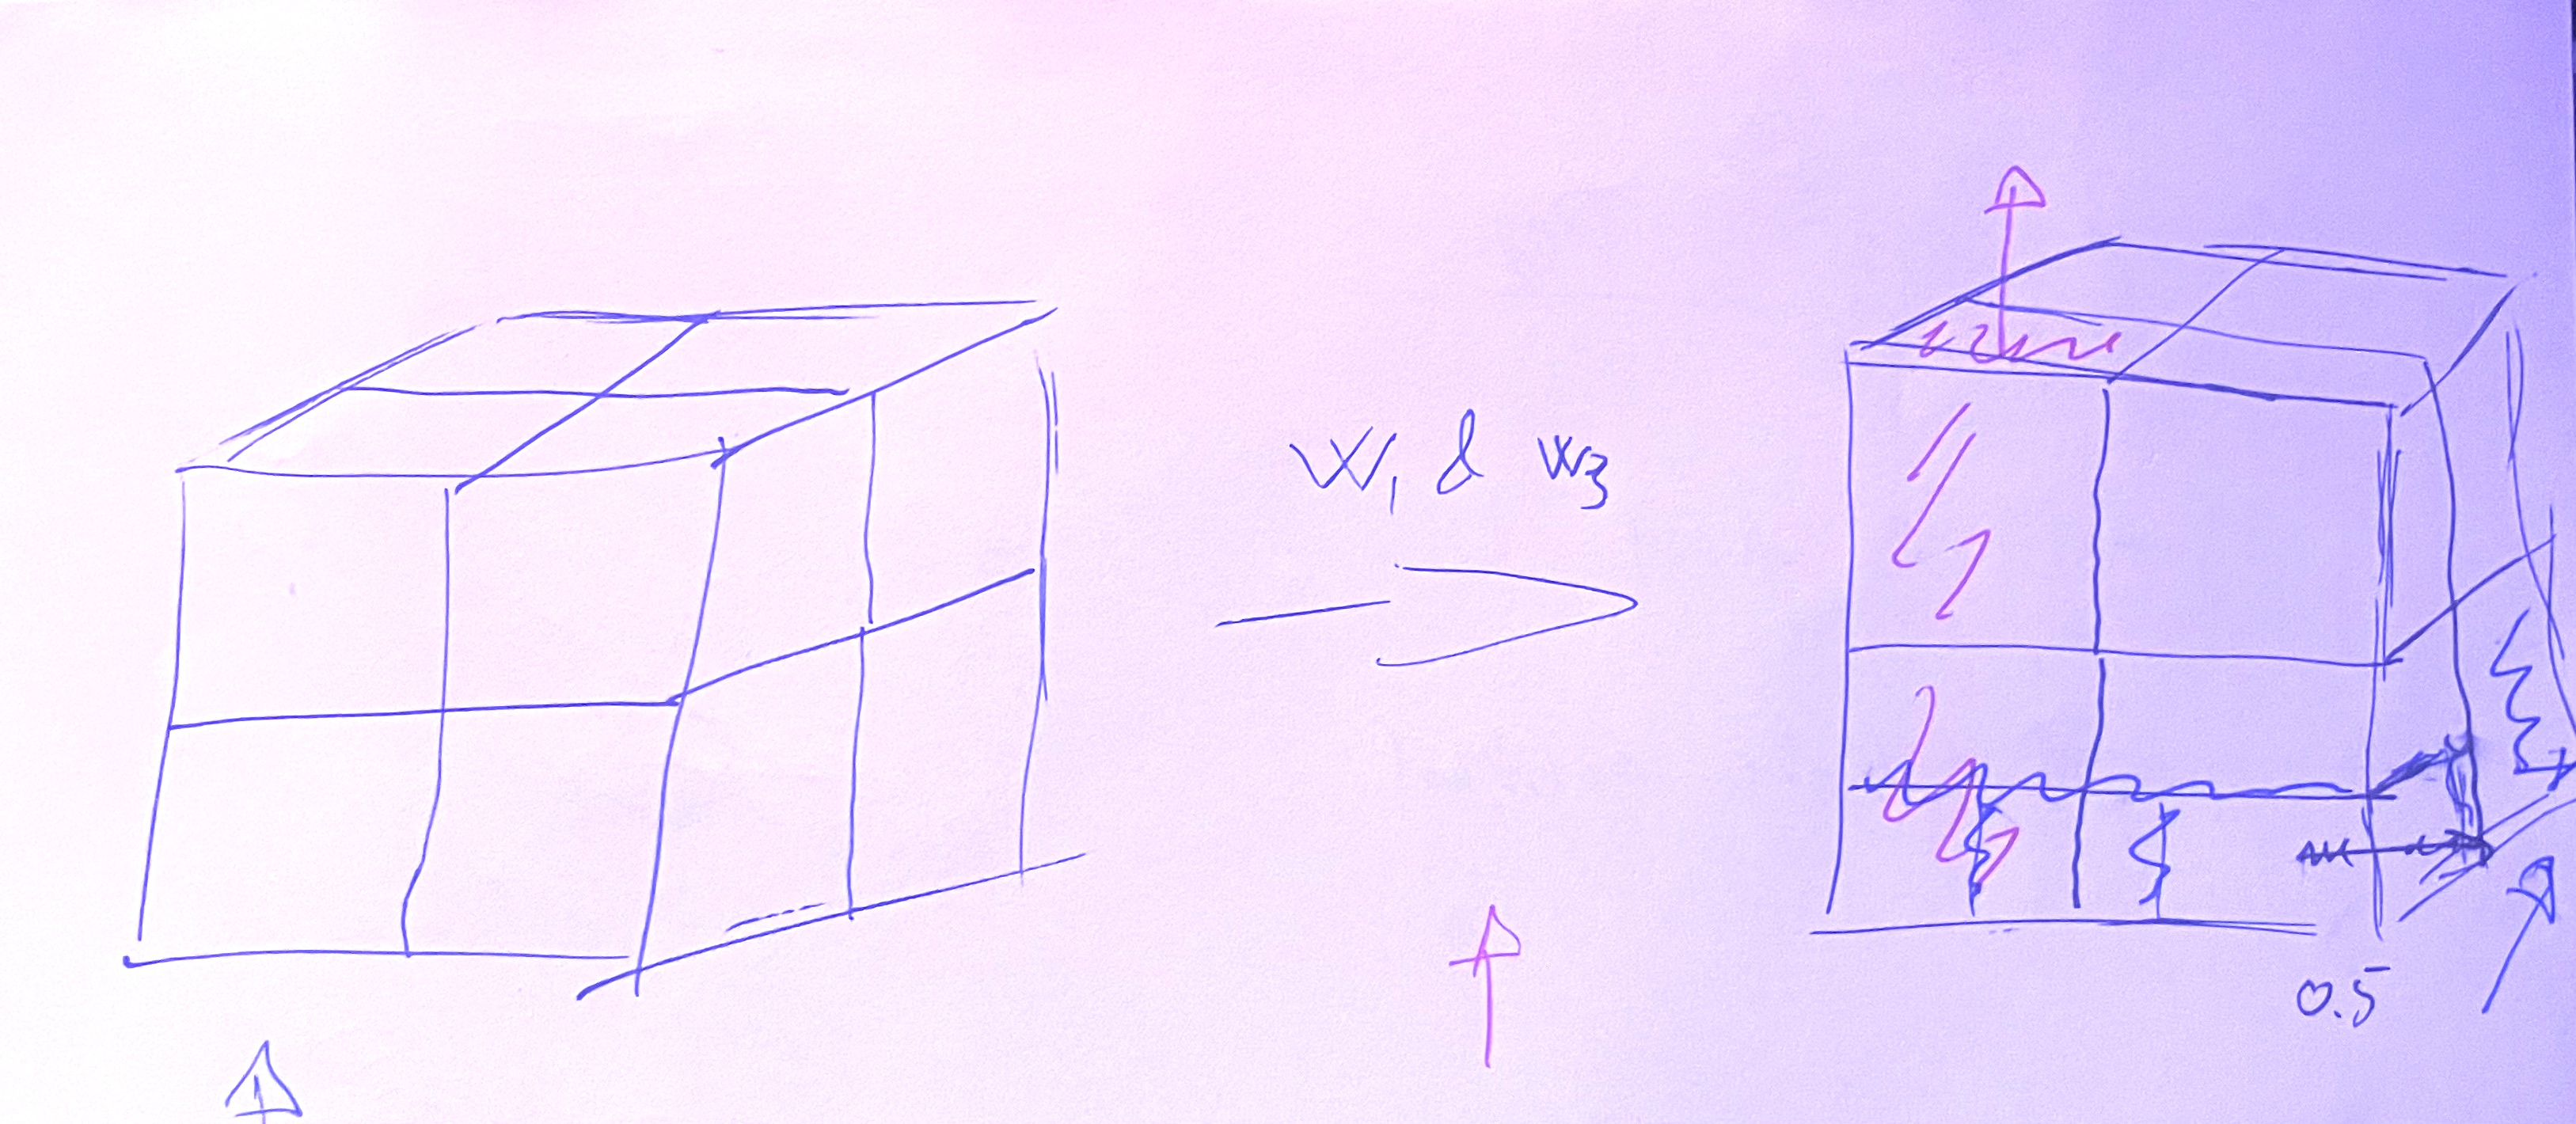
\includegraphics[width=0.87\linewidth]{aper_yeye.jpg}
    %* Figure
    % for the use in the online editor: \usepackage{tikz} 
    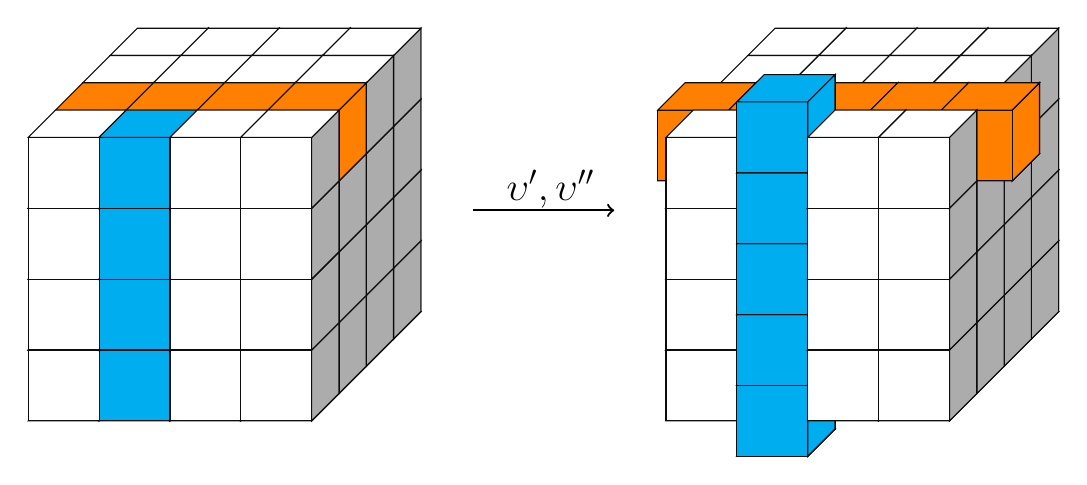
\begin{tikzpicture}[scale=0.9] %! The original scale is 1
        % Define the tile
        \def\tile{
        % Draw the unit cube
            \draw[black!95] (1,0,0) -- (1,0,1) -- (1,1,1) -- (1,1,0) -- cycle; % left face
            \draw[black!95] (0,0,0) -- (1,0,0) -- (1,0,1) -- (0,0,1) -- cycle; % bottom face
            \draw[black!95] (0,0,0) -- (0,1,0) -- (1,1,0) -- (1,0,0) -- cycle; % back face
            \draw[black!95, fill=gray!65] (1,0,0) -- (1,1,0) -- (1,1,1) -- (1,0,1) -- cycle; % right face
            \draw[black!95, fill=white] (0,0,1) -- (1,0,1) -- (1,1,1) -- (0,1,1) -- cycle; % front face
            \draw[black!95, fill=white](0,1,0) -- (0,1,1) -- (1,1,1) -- (1,1,0) -- cycle; % top face
        }

        \def\tilecolumn{
            % Draw the unit cube
                \draw[black!95] (1,0,0) -- (1,0,1) -- (1,1,1) -- (1,1,0) -- cycle; % left face
                \draw[black!95] (0,0,0) -- (1,0,0) -- (1,0,1) -- (0,0,1) -- cycle; % bottom face
                \draw[black!95] (0,0,0) -- (0,1,0) -- (1,1,0) -- (1,0,0) -- cycle; % back face
                \draw[black!95, fill=cyan] (1,0,0) -- (1,1,0) -- (1,1,1) -- (1,0,1) -- cycle; % right face
                \draw[black!95, fill=cyan] (0,0,1) -- (1,0,1) -- (1,1,1) -- (0,1,1) -- cycle; % front face
                \draw[black!95, fill=cyan](0,1,0) -- (0,1,1) -- (1,1,1) -- (1,1,0) -- cycle; % top face
            }
        
        \def\tilerow{
            % Draw the unit cube
                \draw[black!95] (1,0,0) -- (1,0,1) -- (1,1,1) -- (1,1,0) -- cycle; % left face
                \draw[black!95] (0,0,0) -- (1,0,0) -- (1,0,1) -- (0,0,1) -- cycle; % bottom face
                \draw[black!95] (0,0,0) -- (0,1,0) -- (1,1,0) -- (1,0,0) -- cycle; % back face
                \draw[black!95, fill=orange] (1,0,0) -- (1,1,0) -- (1,1,1) -- (1,0,1) -- cycle; % right face
                \draw[black!95, fill=orange] (0,0,1) -- (1,0,1) -- (1,1,1) -- (0,1,1) -- cycle; % front face
                \draw[black!95, fill=orange](0,1,0) -- (0,1,1) -- (1,1,1) -- (1,1,0) -- cycle; % top face
            }
    
        % Draw the tiling pattern LEFT: x = 0,1,2,3
        % not shifted
        % the backseat boys
        \foreach \x in {0,1,2,3}{
            \foreach \y in {-2,-1,0,1}{
                \foreach \z in {-2,-1}{
                    \pgfmathsetmacro{\shiftX}{\x}
                    \pgfmathsetmacro{\shiftY}{\y}
                    \pgfmathsetmacro{\shiftZ}{\z}
                    
                    \begin{scope}[shift={(\shiftX,\shiftY,\shiftZ)}]
                    \tile % Draw the tile
                    \end{scope}
                }
            }
        }
        % Draw the back four cubes as two rows for the shift in X
        % not shifted
        \foreach \x in {0,1,2,3}{
            \foreach \y in {-2,-1,0}{
                \foreach \z in {0}{
                    \pgfmathsetmacro{\shiftX}{\x}
                    \pgfmathsetmacro{\shiftY}{\y}
                    \pgfmathsetmacro{\shiftZ}{\z}
                    
                    \begin{scope}[shift={(\shiftX,\shiftY,\shiftZ)}]
                    \tile % Draw the tile
                    \end{scope}
                }
            }
        }
        % Will be shifted – in the X direction
        \foreach \x in {0,1,2,3}{
            \foreach \y in {1}{
                \foreach \z in {0}{
                    \pgfmathsetmacro{\shiftX}{\x}
                    \pgfmathsetmacro{\shiftY}{\y}
                    \pgfmathsetmacro{\shiftZ}{\z}
                    
                    \begin{scope}[shift={(\shiftX,\shiftY,\shiftZ)}]
                    \tilerow % Draw the tile
                    \end{scope}
                }
            }
        }
        
        
        % not shifted
        \foreach \x in {0}{
            \foreach \y in {-2,-1,0,1}{
                \foreach \z in {1}{
                    \pgfmathsetmacro{\shiftX}{\x}
                    \pgfmathsetmacro{\shiftY}{\y}
                    \pgfmathsetmacro{\shiftZ}{\z}
                    
                    \begin{scope}[shift={(\shiftX,\shiftY,\shiftZ)}]
                    \tile % Draw the tile
                    \end{scope}
                }
            }
        }
        % Draw the front four cubes as two columns for the shift in Y
        % Will be shifted – in the Y direction
        \foreach \x in {1}{
            \foreach \y in {-2,-1,0,1}{
                \foreach \z in {1}{
                    \pgfmathsetmacro{\shiftX}{\x}
                    \pgfmathsetmacro{\shiftY}{\y}
                    \pgfmathsetmacro{\shiftZ}{\z}
                    
                    \begin{scope}[shift={(\shiftX,\shiftY,\shiftZ)}]
                    \tilecolumn % Draw the tile
                    \end{scope}
                }
            }
        }
        % not shifted
        \foreach \x in {2,3}{
            \foreach \y in {-2,-1,0,1}{
                \foreach \z in {1}{
                    \pgfmathsetmacro{\shiftX}{\x}
                    \pgfmathsetmacro{\shiftY}{\y}
                    \pgfmathsetmacro{\shiftZ}{\z}
                    
                    \begin{scope}[shift={(\shiftX,\shiftY,\shiftZ)}]
                    \tile % Draw the tile
                    \end{scope}
                }
            }
        }
        
        % Draw the Inbetween stuff
        %———————————————————————————————————
        \draw[->, thick, black] (5.5,0.2) -- (7.5,0.2);
        \node[black] at (6.6,0.5) {\Large $\upsilon',\upsilon''$}; 
        
        
        
        
        % Draw the tiling pattern RIGHT: x= 9,10,11,12
        %———————————————————————————————————
        % not shifted
        % the backseat boys
        \foreach \x in {9,10,11,12}{
            \foreach \y in {-2,-1,0,1}{
                \foreach \z in {-2,-1}{
                    \pgfmathsetmacro{\shiftX}{\x}
                    \pgfmathsetmacro{\shiftY}{\y}
                    \pgfmathsetmacro{\shiftZ}{\z}
                    
                    \begin{scope}[shift={(\shiftX,\shiftY,\shiftZ)}]
                    \tile % Draw the tile
                    \end{scope}
                }
            }
        }
        % Draw the back four cubes as two rows for the shift in X
        % not shifted
        \foreach \x in {9,10,11,12}{
            \foreach \y in {-2,-1,0}{
                \foreach \z in {0}{
                    \pgfmathsetmacro{\shiftX}{\x}
                    \pgfmathsetmacro{\shiftY}{\y}
                    \pgfmathsetmacro{\shiftZ}{\z}
                    
                    \begin{scope}[shift={(\shiftX,\shiftY,\shiftZ)}]
                    \tile % Draw the tile
                    \end{scope}
                }
            }
        }
        % Will be shifted – in the X direction
        \foreach \x in {8,9,10,11,12}{
            \foreach \y in {1}{
                \foreach \z in {0}{
                    \pgfmathsetmacro{\shiftX}{\x+0.5}
                    \pgfmathsetmacro{\shiftY}{\y}
                    \pgfmathsetmacro{\shiftZ}{\z}
                    
                    \begin{scope}[shift={(\shiftX,\shiftY,\shiftZ)}]
                    \tilerow % Draw the tile
                    \end{scope}
                    
                    %\ifnum\x=9
                    %    \draw[->, orange] (\shiftX+1,1.4) --node[below] {$0.5$} (\shiftX+2,1.4);             \fi
                }
            }
        }
        

        % not shifted
        \foreach \x in {9}{
            \foreach \y in {-2,-1,0,1}{
                \foreach \z in {1}{
                    \pgfmathsetmacro{\shiftX}{\x}
                    \pgfmathsetmacro{\shiftY}{\y}
                    \pgfmathsetmacro{\shiftZ}{\z}
                    
                    \begin{scope}[shift={(\shiftX,\shiftY,\shiftZ)}]
                    \tile % Draw the tile
                    \end{scope}
                }
            }
        }
        % Draw the front four cubes as two columns for the shift in Y
        % Will be shifted – in the Y direction
        \foreach \x in {10}{
            \foreach \y in {-3,-2,-1,0,1}{
                \foreach \z in {1}{
                    \pgfmathsetmacro{\shiftX}{\x}
                    \pgfmathsetmacro{\shiftY}{\y+0.5}
                    \pgfmathsetmacro{\shiftZ}{\z}
                    
                    \begin{scope}[shift={(\shiftX,\shiftY,\shiftZ)}]
                    \tilecolumn % Draw the tile
                    \end{scope}
                    
                    %\ifnum\y=1
                    %    \draw[->, thick, cyan] (7,\shiftY+0.5) --node[right] {$0.5$} (7,\shiftY+1.5);             \fi
                }
            }
        }
        % not shifted
        \foreach \x in {11,12}{
            \foreach \y in {-2,-1,0,1}{
                \foreach \z in {1}{
                    \pgfmathsetmacro{\shiftX}{\x}
                    \pgfmathsetmacro{\shiftY}{\y}
                    \pgfmathsetmacro{\shiftZ}{\z}
                    
                    \begin{scope}[shift={(\shiftX,\shiftY,\shiftZ)}]
                    \tile % Draw the tile
                    \end{scope}
                }
            }
        }
        
        
  
    \end{tikzpicture}
    %\caption{Illisustrated in the \cref{fig:big_aperi} is simply a bigger version of the aperiodic tile we have constructed.}
    %\label{fig:big_aperi}
%\end{figure*}


	% Page setup
	\begin{minipage}{0.4\textwidth}
		\begin{flushleft} \large
			\emph{Author:}\\
			\textrm{\theauthor}
		\end{flushleft}
	\end{minipage}
	\begin{minipage}{0.4\textwidth}
		\begin{flushright} \large
			\emph{\supervisorGrammar:} \\
			\textrm{\supervisorA}\\  % Supervisor #1
			\textrm{\supervisorB} %\\  % Supervisor #2
			%\textrm{ } %\\  % Supervisor #3
		\end{flushright}
	\end{minipage}\\[1.5 cm]
	

	{\large \thedate}%\\[2 cm]
 
	%\vfill

\end{titlepage}

  % title for max titlepage

    %\setcounter{tocdepth}{2}
    \tableofcontents
    \printglossaries


    % --- DOCUMENT START --- %
    % --- NOTE: Folder structure --- %
    % Allows compilation of each subfile, rather to compile everything at once
    % Subfiles must have this file as option while using the documentclass subfile
    % Loading a subfile is done with \subfile{"path-to-file"}
    % ---
    \ifSaveGit  
        \chapter{Lorum Intro}
            \subfile{chapters/xx_lorum_chap_1.tex}
            %\subfile{chapters/introduction.tex}  % NTNU info 
    \else
        \chapter[]{Intro?}
            \subfile{chapters/01_introduction.tex}

        \chapter{The complex trigonometric system}
            \subfile{chapters/02_cmplx_trig_system.tex}
            \subfile{chapters/021_cmplx_trig_system.tex}
    \fi

    %\chapter{Intro?}
    %    \subfile{chapters/01_introduction.tex}
%
    %\chapter{The complex trigonometric system}
    %    \subfile{chapters/02_cmplx_trig_system.tex}
    %    \subfile{chapters/021_cmplx_trig_system.tex}



    \printbibliography
    % Bibliography old
    %\bibliographystyle{preamble/AGFstyle.bst}
    %\bibliography{preamble/Mastergrad!.bib}

\end{document}
